\documentclass[a4paper,fleqn]{cas-dc}

% If the frontmatter runs over more than one page
% use the longmktitle option.

%\documentclass[a4paper,fleqn,longmktitle]{cas-dc}

%\usepackage[numbers]{natbib}
%\usepackage[authoryear]{natbib}
\usepackage[authoryear,longnamesfirst]{natbib}

%%%Author macros
\def\tsc#1{\csdef{#1}{\textsc{\lowercase{#1}}\xspace}}
\tsc{WGM}
\tsc{QE}
%%%

% Uncomment and use as if needed
%\newtheorem{theorem}{Theorem}
%\newtheorem{lemma}[theorem]{Lemma}
%\newdefinition{rmk}{Remark}
%\newproof{pf}{Proof}
%\newproof{pot}{Proof of Theorem \ref{thm}}

\begin{document}
\let\WriteBookmarks\relax
\def\floatpagepagefraction{1}
\def\textpagefraction{.001}

% Short title
\shorttitle{TEMPORARY TITLE}    

% Short author
\shortauthors{White, Dahl, Orton}  

% Main title of the paper
\title [mode = title]{Investigating Jupiter's Atmosphere Through Near-Infrared Thermal Imaging and Spectral Analysis}  

% Title Choices: 

% Title footnote mark
% eg: \tnotemark[1]
\tnotemark[1] 

% Title footnote 1.
% eg: \tnotetext[1]{Title footnote text}
\tnotetext[1]{Title Footnote} 

% First author
%
% Options: Use if required
% eg: \author[1,3]{Author Name}[type=editor,
%       style=chinese,
%       auid=000,
%       bioid=1,
%       prefix=Sir,
%       orcid=0000-0000-0000-0000,
%       facebook=<facebook id>,
%       twitter=<twitter id>,
%       linkedin=<linkedin id>,
%       gplus=<gplus id>]

\author[1]{Kennedi J. White}[type=editor,
       orcid=0000-0000-0000-0000]
\cormark[1]
\fnmark[1]
\ead{}
\ead[url]{}

% Credit authorship
% eg: \credit{Conceptualization of this study, Methodology, Software}
\credit{}

\affiliation[1]{organization={Department of Physics and                Astronomy, Howard University},
            addressline={2355 6th St., NW}, 
            city={Washington},
            postcode={20059}, 
            state={D.C.},
            country={USA}}

\author[2,3]{Emma K. Dahl}[type=editor,
       orcid=0000-0000-0000-0000]
\fnmark[2]
\ead{}
\ead[url]{}

% Credit authorship
\credit{}

\author[2]{Glenn S. Orton}[type=editor,
       orcid=0000-0000-0000-0000]
\fnmark[2]
\ead{}
\ead[url]{}
\credit{}

\affiliation[2]{organization={Jet Propulsion Laboratory},
            addressline={4800 Oak Grove Dr}, 
            city={Pasadena},
            postcode={91109}, 
            state={CA},
            country={USA}}

\affiliation[3]{organization={California Institute of Technology},
            addressline={4800 Oak Grove Dr}, 
            city={Pasadena},
            postcode={91109}, 
            state={CA},
            country={USA}}

% Corresponding author text
\cortext[1]{Corresponding author}

% Footnote text
\fntext[1]{}


\begin{abstract}
THIS ISN'T ACTUAL ABSTRACT
This project, operated remotely through the Jet Propulsion Laboratory (JPL), focused on reducing and analyzing the near infrared thermal images and spectra of Jupiter. Images of gaseous planets, in this instance Jupiter, are sensitive to various atmospheric parameters such as temperature, presence of molecules, and the opacity of the clouds. Investigating these parameters at different near-infrared wavelengths can reveal interesting scientific phenomenons within Jupiter’s atmosphere. By reducing the images of Jupiter at different wavelengths, its atmospheric properties can be determined; particular interest and focus were on the clouds in the atmosphere and their properties.

\end{abstract}

\begin{highlights}
\item 
\item 
\item 
\end{highlights}


%\nocite{*}

% Keywords
% Each keyword is seperated by \sep
\begin{keywords}
EZ Disturbance \sep Jupiter \sep Planetary Science \sep
\end{keywords}

\maketitle


\section{Introduction}
% Jupiter's clouds overview
Jupiter is our Solar System’s largest gas giant and is most recognizable by its horizontally thick banded clouds that persist in the atmosphere. Its clouds are characterized by alternating bands of different colors and properties. Nominally, Jupiter's bands are separated into six belts split between the north and south and seven zones split between the north, south, and equator. The belts are typically dark colored, lower altitude regions where characterized by descending air patterns. This limits cloud formation in the area, causing deeper, darker cloud layers that can be more turbulent (\cite{bagenal2006jupiter}). The zones are lighter colored, high altitude regions primarily characterized by rising air that forms ammonia (NH$_3$) ice clouds (\cite{bagenal2006jupiter}). They are typically cooler and more stable than belts due to the zonal flow of gases underlying the zone. These alternating belts and zones create a distinct patterned appearance and are normally 'held in place' by Jupiter's zonal jet streams. However, Jupiter's atmosphere undergoes a unique phenomenon that can disrupt its appearance (\cite{bagenal2006jupiter}). 

% Jupiter's atmosphere changes a lot
Jupiter's atmosphere contains complex storm systems and turbulence that affect its appearance (CITATION). These storms can last to hundreds of years (CITATION). One of its more well-known storm systems is the Great Red Spot (GRS), a supermassive anticyclonic storm (CITATION). The planet also displays some transient phenomenons like hot spots in clear, warmer regions and thunderstorms. Atmospheric waves like Rossby and Kelvin waves further contribute to the dynamic nature of Jupiter's weather, while periodic oscillations of gaseous jets, such as the Quasi-Quadrennial Oscillation, cause variations in equatorial temperatures and wind patterns (CITATION). The aforementioned atmospheric weather events are well-known and documented (CITATION). As of late, another Jovian weather event, an enigmatic disturbance that occurs in the Equatorial Zone (EZ), has warranted further study to understand what makes this disturbance appear differently than others and what dynamics caused the disturbance to present.

\section{Background}
% EZ disturabnces
Jupiter’s EZ is generally located between ~15\textdegree N and ~15\textdegree S. with the GRS dominating the lower section of the south Equatorial Zone (EZs) from ~10\textdegree S and ~15\textdegree S. The EZ displays quasi-periodic patterns of NH$_3$ ice-rich white plumes and dark formations. Termed 5-$\mu$m hot spots, the openings in the cloud deck from these plumes are visible due to their brightness at this wavelength. These features are typically confined to pressures below 8 bar due to the limited depth visible in the cloud openings. At 5 $\mu$m, the EZ typically appears uniformly dark due to thick NH$_3$ ice clouds, except at its northern boundary where hot spots are found.\citep{antunano2018infrared} found that the EZ undergoes a quasi-periodic disturbance every 6-8 or 13-14 Earth years, significantly altering its appearance in infrared and visible wavelengths. During these disturbances, the EZ typically develops a narrow 5-$\mu$m-bright band and a wave-like pattern with bright filaments. These events often feature variable dark festoons emerging from hot spots, accompanied by white plumes as seen in 5-$\mu$m \citep{antunano2018infrared}. The EZ variability shows periodicity at visible wavelengths (8 years) and ultraviolet (12 years) (CITATION). These disturbances can last 1–1.5 years and begin about 18 months after the EZ's coloration changes visibly \cite{antunano2020characterizing}. Such disturbances have been explored through the use of archival images from 1973, 1979, 1992, 1999, 2006, and 2018 \cite{antunano2020characterizing, 2022DPS....5420501D, 1994JGR....99.8425S, 1988Icar...76..533S}. 

% EZ distuarbance from 2018-2022 and why it's weird
As stated, the EZ is characterized by upwelling where NH$_3$ forms a continuous cloud layer up to the 700-mbar level; Discrepancies in the opacity of these deep clouds can affect our understanding of the EZ and the disturbances that occur in that region. In 2018, an unusual EZ disturbance began that featured a decrease in opacity of these deep clouds and a lack of cloud clearing \cite{orton2019juno}. This same disturbance did not display the dramatic cloud-clearing and brightening at 5-$\mu$m as past disturbances. Increased 5-$\mu$m brightening failed to appear consistently. When 5-$\mu$m streaks were found they were not sustained for long periods of time \cite{orton2019juno}. The EZ then returned to nominal conditions around 2022 (\cite{2023DPS....5532605D}). Studying this particular disturbance, which is unique compared to those studied in the past, the Jovian atmospheric evolution can be better understood. A variance in the 'types' of disturbances studied can help inform initial parameters for other Gas Giants in our Solar System and exoplanetary systems, in addition to expanding our knowledge on disturbances in general.

% Paper summary and goals
We set out to characterize the most recent EZ disturbance with respect to the cloud formation and placement in the atmosphere. The 2018-2022 EZ disturbance haze evolution presents a loft at 2.16 $\mu$m suggesting a correlation between the haze and the discrepancies in the disturbance (\ref{fig:haze-evolution}). Modeling this haze loft can inform what parameters caused this, and potentially what caused the changes in the recent EZ disturbance. In Section 3, we discuss the data reduction and extraction necessary to run the models used in this study. Section 4 briefly reviews the radiative transfer methodology, followed by the results and analysis in Section 5 and 6, respectively. 

\begin{figure}
    \centering
    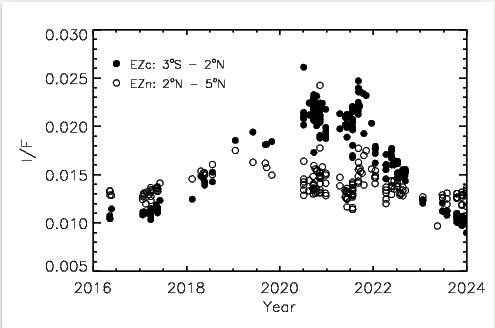
\includegraphics[width=1.0\linewidth]{haze_evolution.png}
    \caption{A lofted haze at 2.16 microns between 2019 and 2023.}
    \label{fig:haze-evolution}
\end{figure}

\section{Methodology}
% Brief description of whats used for observation & reduction
Our investigation of the Jovian atmosphere relies on the archival data provided by SpeX, a medium-resolution spectrograph operating in the 0.8-5.4-$\mu$m range, on the NASA InfraRed Telescope Facility (IRTF). Examining Jupiter in the near-infrared spectrum enables the correlation and interpretation of events across various wavelengths. Infrared observations prove crucial in detecting substantial plumes of denser gaseous molecules, directly linking them to visible attributes like color plumes and upper atmospheric waves (CITATION). These findings will contribute to our comprehension of the weather patterns on the largest planet in our solar system.

\subsection{Observation}
Jupiter has unexplained disturbances in its atmosphere every six to eight or thirteen to fourteen Earth years (\citep{antunano2018infrared}). Observing these disturbances can be difficult to view in the visible spectrum. When viewing Jupiter’s atmosphere in the infrared, however, interesting atmospheric events can more easily be recorded. The IRTF on Mauna Kea, Hawaii was used to capture images of Jupiter. The atmospheric data collects Jupiter’s internal dynamics; they are used to predict and analyze the regions of interest, notably, the EZ. The images undergo standard data reduction procedures, including A/B subtraction and flat division, in the IDL-based Data Reduction Manager (DRM) program . The reduced data can serve various purposes such as identifying wave patterns to tracking features like the Great Red Spot. The IRTF's archive of Jupiter’s data was used to study the long-term temporal patterns in the planet's atmosphere. A periodic trend in the waves in the North Temperate Latitudes was found; this is linked to an expansion in the North Equatorial Belt.

There was a focus on reducing and analyzing the near-infrared (1.22-3.80 $\mu$m) thermal images of Jupiter. The images are sensitive to various atmospheric parameters such as temperature, presence of molecules, and the opacity of the clouds. Investigating these parameters at different near-infrared wavelengths revealed significant atmospheric (CITATION). We narrowed in on the clouds in the atmosphere and their properties as a means to explore these disturbances. These images are then reduced, formatted, and put into an atmospheric retrieval code to derive and simulate the opacity of the clouds. 

\subsection{Data Reduction and Spectra Extraction}
The Bergman and Waldram (CITATION) reduction method was used to produce the SpeX images needed for the atmospheric retrieval code. Multiple near infrared images were collected at wavelengths 1.22 $\mu$m - 3.80 $\mu$m in the form of planet (‘A’) and sky (‘B’) images (CITATION). The data reduction manager (DRM) for planetary data image reduction was used and accessed through IDL.

A flat field –an image of the background sky– and a bad pixel mask –an image used to smooth over the dead pixels– that corresponds to the date and wavelength of the image paths are retrieved and loaded into the DRM. Images are in numerical order following the ‘ABAB’ naming patterns of the file. Once all target images are acquired, in the ‘ABAB’ order in numerical order, the ‘B’ images are subtracted from the ‘A’ images. Only ‘A’ images will be left. Using the appropriate flat field, the ‘A’ images are divided by the flat field. The reduced images are browsed to discern which are the best to be co-added together. 

At this stage, the ‘A’ images are despiked to get clearer images before co-adding. Any unclear or cut off images are removed. The selected images are then co-added using the bad pixel mask to create one overlaid image. This image is flipped to reverse the optical inversion of the planet done by the telescope. At this stage, which molecules are more prevalent at which wavelength based on the atmospheric depth brightness can be distinguished and noted. In its raw state the images can be too bright or dark; The initial image brightness is altered for accuracy and the co-added image can be despiked for clarity prior to being saved (CITATION). After images are reduced, they need to be calibrated for the best results during analysis. The saved image undergoes a geometry fit limb to assign latitudes, longitudes, and emission angles to the data. The disk aperture photometry is then recorded and applied by the expression
\begin{equation}
\frac{a*R_a}{P_a} 
\end{equation}
with $R_a$ being the disk averaged reflectivity and $P_a$ as the disk averaged pixel count. 

Cylindrical, $\mu$, and $\mu_0$ maps were created and saved to convert the radian numerical data into I/F spectra (CITATION). These maps are put into an atmospheric retrieval code (Emma CITATION) resulting in an I/F plot (graphs the change in I/F across wavelengths on a given day), an I/F spectra text file (the wavelengths with their corresponding I/F), and a .spx file (the initial inputs to analyze Jupiter’s atmospheric profile). 

The cylindrical, $\mu$, and $\mu_0$, maps are added to a historical Jupiter haze scatter plot separated by wavelength. This plot assess the change in the opacity of the clouds over time and the effects each wavelength's chemistry has on the haze. As stated in Sec. 2, the added plot points are used to record the change in Jupiter’s atmospheric haze during and after a disturbance event. The addition of the 2023 data showed a steady decrease in the EZn back to what it was in 2016. This followed a spike in haziness from 2018 to 2020. In the EZc there was a relatively linear amount of haze with a maximum in 2021 and additional data from 2021 (\ref{fig:haze-evolution}).

\section{Radiative Transfer Modeling}
NEMESIS, an estimation retrieval algorithm, was used to gather the atmospheric profile that best fits what is occurring in the atmosphere based on the data. It analyzes which atmospheric chemistry is affecting the atmosphere the most in the target wavelengths (CITATION). A priori guesses for the cloud parameters are set up for each run. The NEMESIS modeling will use two Gaussian clouds with total optical depth, peak pressure, and full width half maximum (FWHM) in pressure space for the cloud parametrization. Cloud parametrization was made with the intent to constrain the location of the planetary haze over multiple wavelengths. When a parametrization is decided, the a priori guesses are kept the same for each run so that the start is at the same point for each observation.



Main cloud will be mostly set and won’t vary; we want that input to be constant over time bc we’re interested in the haze properties changing)
Analyze results by examining reduced chi squared value (e.g. goodness of fit), how the 3 parameters of the haze change over time
If the reduced chi squared is way off, consider letting input parameters vary a bit more

\section{Results}

\section{Post-Model Analysis}

\bibliographystyle{cas-model2-names}
\bibliography{sample}

\end{document}


